\chapter{Theoretical Appendix A: Model theory and statistical methods}

\section{Model Theory}
This thesis is concerned with a particular kind of scientific model: those that are subject to mathematical analysis, and tractable subjects for numerical simulation techniques. Most biological models do not fit this description, but increasing computing power has expanded the potential for, in particular, cellular and macromolecular explanations to be formalized and tested in this way. While doing so is sometimes derided as ``physics envy'', the reality is more complex. Simple heuristics are, sometimes, adequate biological explanations; much of differential diagnosis consists of reliable descriptive relations between qualitatively characterised signs in patients, and the presence of a pathogen, for instance. More often, the complexity of biological systems, and the sophistication of the instruments with which we probe them, give rise to observations which support more than one plausible causal explanation for the features of the data. The question of model comparison then immediately arises. Without numerical analysis, we may only make reference to the use of the model in applied domains where the model failure has commercial consequences. Because biological models are rarely required to succeed as engineering tools, for the prediction and control of outcomes of practical significance, an inability to analyse them numerically means that we are left only with rhetoric to assess their relative explanatory value. This approach to ``model comparison'' necessarily devolves into the anarchic Feyerabendian discursive chaos discussed in \autoref{sec:Feyerabend}. Feyerabend correctly points out that scientific models can only be compared against one another, and that the selection of comparative criteria can never be ``objective'' in the sense of being fully independent of the contingent situation and goals of the observer. Nothing can be done about this; either we look for relatively-better criteria and relatively-better models as judged by those criteria, or we remain in the realm of pure metaphysical rhetoric, without investigating their implications, what Feyerabend describes as the realm of the ``crank'':

\begin{longquote}
[T]he distinction between the crank and the respectable thinker lies in the research that is done once a certain point of view is adopted. The crank usually is content with defending the point of view in its original, undeveloped, metaphysical form, and he is not prepared to test its usefulness in all those cases which seem to favor the opponent, or even admit that there exists a problem. It is this further investigation, the details of it, the knowledge of the difficulties, of the general state of knowledge, the recognition of objections, which distinguishes the ‘respectable thinker’ from the crank. The original content of his theory does not.
\cite[pp.199]{Feyerabend1981}
\end{longquote}

The support of complex biological systems for multiple explanations often gives rise to calls for explanatory pluralism \cite{Brigandt2010}. It should be emphasized that very differently parameterised models can be adequate explanations for the same system. This is particularly common for explanations at different descriptive depths. For instance, the models used in \autoref{chap:CMZ} make no reference to particular macromolecules, but we would still like to have macromolecular explanations of RPC function, particularly because these may supply us with means to intervene onto RPC proliferative and lineage outcomes. In other plural explanations, adequate, differently-parameterised models of the same system may be describing different aspects of the same level of organization. Pharmacological kinetic studies of G-protein association with receptors, and crystallographic studies of the same phenomenon, are a good example. These models allow experimenters to pursue different descriptive and interventional objectives. Indeed, as Nicholas Rescher has noted, attempts to synthesize many models into a single overarching explanation often result in descriptive chaos \cite[p.65-6]{Rescher2000}. Rescher explains how the descriptive adequacy of some model in its local domain usually requires the blurring out of at least some pertinent details of the system that could have been included; it can be added that the the computational tractability of the model requires the same.

If we virtually all accept this form of pluralism, we are still left with the cases where models are making contradictory claims about reality\footnote{That is, they have incompatible metaphysical content; they are therefore subject to counterinduction as explained in \autoref{sec:Feyerabend}}. Pluralism cannot coherently extend to abandoning the fundamental logical law of non-contradiction, without compromising the entire endeavour of scientific rationalism. We cannot accept logically contradictory notions about the structure of reality without precluding cognitive harmony arising from a broadly consistent view of the way the world works \cite{Rescher2005}. Given the complexity of biological systems, we have no option except to express models formally and to test them rigorously against one another. This is the task of model selection.

Model selection requires that we be able to score models against observational datasets encoding the phenomena they represent, to measure their quality. This requires the selection of a quality function. Loss functions, like \hyperref[AIC]{AIC}, used in \autoref{chap:SMME}, express the relative amount of information in the dataset lost by the model, given a set of parameters. Likelihood functions, used elsewhere, express the likelihood of the data given the model and parameters. The parameters of the model thus define an n-dimensional ``parameter space''; the quality function expresses a hypersurface within this space. By sampling within this space, we may estimate the shape of the surface. This sampling information can be used in three ways: we may propose new, higher quality parameter space locations to sample from, in search of the highest quality parameterisation of the model (\hyperref[opt]{model optimisation}); we may derive marginal likelihoods for particular parameter values (\hyperref[est]{parameter estimation}), or we may estimate the quality of the model over all parameterisations (\hyperref[evi]{evidence estimation}). These topics are discussed below.

\subsection{Bayesian Epistemological View on Model Comparison}
\label{ssec:BayesEpistemology}
The analyses presented in the data chapters express two views on how model comparison should be approached. The first, expressed in \autoref{chap:SMME}, is drawn from information theory, while the second, taken up in \autoref{chap:CMZ}, is a relatively conventional Bayesian view, albeit with more sophisticated tools and more computing power than has been available to Bayesians in the past. In the same way that frequentist analyses may be expressed as a subset of Bayesian analyses (i.e. they normally seek the maximum a priori model parameterisation and likelihood from uninformative priors), informational theoretical approaches to model comparison can be expressed as a subset of Bayesian model comparison theory. In fact, the loss function used in \autoref{chap:SMME}, \hyperref[AIC]{Akiake Information Criterion}, has been adapted to refer to a prior distribution, as the Bayesian Information Criterion \cite{Posada2004}. The intent of these criteria is to take Occam's Razor to the maximum-likelihood approach by penalizing the maximum-likelihood value (or maximum a priori score, in the case of BIC) by the number of free parameters.

The general approach of optimizing a model for a quality against a dataset, then penalizing the best model quality by the parameterisation of the model, allows us to overcome the most important problem with maximum-likelihood approaches to model selection: the requirement for models to be parametrically nested. Model nesting precludes \hyperref[sec:Feyerabend]{counter-induction}; we cannot compare the adequacy of models which express fundamentally different views of how the described system is parameterised, only whether adding more parameters improves a particular view. Escaping this limitation is what allows us to compare stochastic and deterministic mitotic mode models in \autoref{chap:SMME}; these models express different views of how reality is organised. Still, in important ways, this approach shares the basic problem of simply calculating the \hyperref[ssec:MLE]{MLE}: the score in no way accounts for the relative robustness of the model fits. That is, a model which is a terrible description of a dataset over most of its plausible parameter space, but an excellent one in a tiny region, can appear to be a better explanation than a model which is a broadly good description over the whole parameter space. Simply using the number of parameters to penalize the best model found in some sampling procedure fails to express the extent to which the inclusion of those parameters is justified by improving the overall likelihood of sampled models.

This leads us to what may be regarded as the completion of the Bayesian view on model selection\footnote{If nested sampling is not \textit{the} completion of the Bayesian system, it is at least \textit{a} complete Bayesian system.}, John Skilling's system of Bayesian inference, \hyperref[ssec:nested]{nested sampling} \cite{Skilling2006,Skilling2012,Skilling2019}. By rearranging the usual presentation of Bayes' rule, Skilling reveals how it specifies the computational inputs and outputs associated with the activities of model sampling, parameter estimation, and evidence estimation. Bayes' rule is typically written as follows, where $x$ is a logical proposition about the data (e.g. specific values for the cell cycle length and exit rates of the CMZ), and $Pr(a|b)$ denotes the probability of a given b:

\[Pr(x|data) = \frac{Pr(data|x)Pr(x)}{Pr(data)}\]

This can be read aloud as "the posterior probability of the proposition, given the data, $Pr(x|data)$, is equal to the likelihood of the data, $Pr(data|x)$, given the proposition, multiplied by the prior probability of the proposition, $Pr(x)$, and divided by the marginal probability of the data over all such propositions, $Pr(data)$." This gives the impression that the principal task in statistical analysis is the calculation of the posterior probability of a model, and gives rise to the treatment of the marginal probability, $Pr(data)$, as a mere normalizing constant. Skilling rearranges this to put computational inputs on the left, and outputs on the right:

\[Pr(x)Pr(data|x) = Pr(data)Pr(x|data)\]

This shows us that the evaluation of a model consists of supplying a prior probability for the proposition, $Pr(x)$, and a likelihood function to assess the probability of the data given that proposition, ($Pr(data|x)$). In return we receive, as computed output (over many propositions $x$) the total evidentiary mass of the data for this model, ($Pr(data)$), as well as the posterior parameter estimates, $Pr(x|data)$. Sample model parameters are drawn from the prior; the likelihood of this proposition about the data is calculated. By accumulating many such samples, the marginal probability of the model over all of these propositions (the evidence for the model) can be estimated. Because these samples may be weighted by their calculated likelihoods and position on the prior, we may also use them to estimate the marginal posterior probabilities of parameters of interest. 

This encapsulates both the numerical procedures involved in model analysis, as well as the epistemological view implied by Bayesian statistics. That is, a model analysis is the joint product of the model and the data, which expresses our belief about the overall credibility of the model ($Pr(data)$)\footnote{ie. a better model gives higher marginal probability to observations than a worse one}, as well as allowing us to estimate the distribution of credibility we should assign to various values for parameters of the model (propositions), $Pr(x|data)$. These are the two fundamental levels on which quantitative measurements of natural systems allow us to make inferences. We may distinguish between models of the systems in a general sense by their evidence, when applied to the same overall dataset. This allows us to counterinductively test contradictory descriptions of the structure of the phenomenon against one another, inferring which is a better map to the territory. The second level of inference is the ranking of propositions for the parameterisation of models achieved by the sampling procedure. This allows us to determine which particular propositions about the system are supported, given the model. Because the posterior distributions need not be unimodal, we can evaluate these modes as separate hypotheses that are supported to varying degrees by the data. 

This view dispenses with problematic interpretations of model selection as being about finding the ``true model'' of reality, or of estimating the actual, objective probabilities inhering in things or processes (a view disputed in \autoref{sec:chance}). Instead, we are guided to focus on the relative quality of models in explaining all of the relevant data we can gather; we may then evaluate the relative quality of specific propositions about the system within those models (i.e., the posterior distributions on model parameters) as we see fit.  

\subsection{Model sampling and optimization}
\label{sampleoptim}
There are now many techniques used to sample the parameter space of a statistical model, given a quality function which scores the model. These have a variety of purposes. Commonly, one wishes to ``optimize'' a model by finding the parameter vector which produces the best objective function result, given some dataset. This is often referred to as Maximum Likelihood Estimation, the product being a Maximum Likelihood Estimate, with MLE used to refer to these interchangeably. \hyperref[ssec:SPSA]{SPSA} is used in this thesis to optimize cell-based models of RPC activity in \autoref{chap:SMME}. The likelihood scores are penalized by the number of model parameters to produce an \hyperref[ssec:AIC]{AIC} score. MLE methods are broadly useful for many applications, with some tuning. SPSA is used in control systems, to maintain the consistency of modelled processes by estimating the inputs most likely to achieve a setpoint, for instance. More sophisticated applications of sampling involve the estimation of the distribution of quality values over the parameter space, rather than focusing solely on estimating the optimal value.

The process of model sampling requires a type of algorithmic logic additional to the quality function, which is a means to generate proposed parameter vectors to be supplied to the function. Most effective sampling methods operate by performing an initial sample from some type of prior information\footnote{In the SPSA optimization performed in \autoref{chap:SMME}, this took the form of the original, poorly optimized fit for the stochastic model and a best guess for a related vector for the deterministic model. In subsequent nested sampling analyses, initialization is performed by sampling randomly from a defined prior distribution.}, and then iteratively generating new proposals from these initial ones. This iterative proposal generation forms a chain of linked positions within parameter space. Generally, new proposals are made considering information related only to the last accepted proposal\footnote{Proposal rejection can occur for a variety of reasons, depending on how the parameter space is interpreted. In Galilean Monte Carlo, this occurs if proceeding along the specified velocity vector would produce a proposal less probable than the last one.}. Because the process is ``memoryless'' in the Markovian sense, and involves the iterative generation of models, it is often called Markov Chain Monte Carlo (MCMC).

Many algorithms for proposal generation exist, and the success of any sampling procedure depends on their properties. Most offer a physical interpretation of the surface formed by the quality function in parameter space. Basic random-walk proposal generation, like the original Metropolis-Hastings implementations of MCMC, is often too inefficient to be usable for high-dimensional parameter spaces, and has broadly been replaced by these physical sampling methods. \hyperref[ssec:SPSA]{SPSA}, for instance, is a simple gradient method. New proposals are generated by bracketing an existing sample with a pair of samples that define an $n$-dimensional ``slope'' at the current location. By proposing a new location up-slope, we receive a new sample which is closer to the local optimum, and we may inexorably approach it in this way. Other, more sophisticated interpretations seek to fix problems with random-walk proposal generation by mechanical interpretations of proposal movement through parameter space, like Hamiltonian Monte Carlo, or thermodynamic interpretations, like simulated annealing. These methods are better suited to the estimation of the distribution of objective function values than an algorithm like SPSA.

In order to ensure the accuracy of any such estimated distribution across parameter space, the algorithm should, ideally, produce proposals in ``detailed balance'', which refers to the physical concept of reversibility found in classical mechanics. The purpose of constraining proposal generation in this way is to guarantee that particular areas of the parameter space are not over- or under-sampled, distorting the final estimate, as a consequence of the manner in which the sampling algorithm generates proposals. \hyperref[ssec:GMC]{Galilean Monte Carlo} has the property of being in detailed balance.

\subsection{Overfitting}
\label{ssec:overfit}
Overfitting is among the most common problems in statistical modelling. This can arise from an unjustified excess of model structure relative to the information present in the data. This excess structure allows the model to capture measurement noise in the dataset the model is being scored against. This gives the appearance of a model which is highly explanatory, but which reflects the particular structure of the measurement errors in the training data better than the overall phenomenon. This problem will typically become apparent in cases of sequential inference; an overfit model will fail to explain new observations as well as it explained previous ones.

A second source of overfitting is the failure to properly account for uncertainty and prior information. For instance, if a unidimensional measurements are modelled with a Normal Gaussian distribution, the MLE Normal Gaussian (whose parameters arise from calculating the mean and standard deviation of the measurements, given the assumption of Normality) can be an overfit to the data. In this simple example, this usually means that the MLE Normal is overly influenced by ``outliers''. This is one case of the general overfitting problem seen in MLE methods \cite{Green2017}. Accounting for available prior information is the best solution to this problem. As this thesis demonstrates, appropriate accounting for our uncertainty about the parameters of the Normal model, and comparison of the Normal case with appropriate alternatives that might better reflect the underlying causal structure that produces the ``problem'' data (in this case, Log-Normal models), both help in producing more accurate estimates of model parameters.
 
\subsection{Simple Stochastic Models}
\label{ssec:SSM}

\begin{figure}
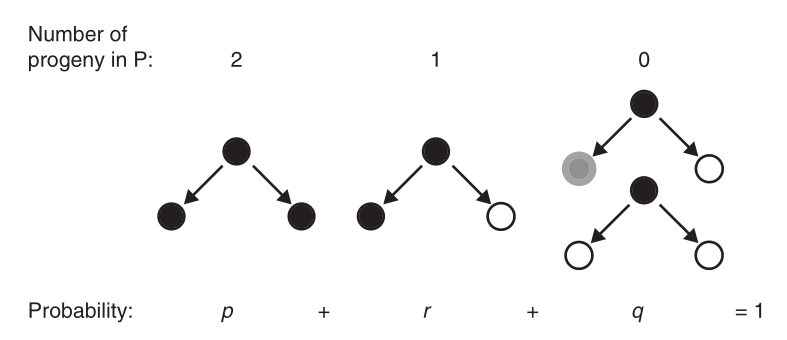
\includegraphics[scale=.5]{simplestochasticmodel}
\centering
\caption{Simple stochastic stem cell model, representing probabilities of cell division events, excerpted from Fagan 2013 pg. 61. Black circles denote proliferative cells, while white and grey circles denote different types of postmitotic offspring. ``Number of progeny in P" is the number of mitotic offspring produced by each type of division. The probability of each division type must sum to 1, as all possibilities are represented, granting that the division types are defined by the postdivisional mitotic history of the offspring.}
\label{fig:SSM}
\end{figure}

The Simple Stochastic Model is schematically summarised in Figure \ref{fig:SSM}. This is the basic structure of the great majority of formal models in the stem cell literature, derived from post-hoc analyses of populations taken to include stem and progenitor cells. The population-level approach is usually explicit, as no differentiation is made between types of proliferating cell- in general, no particular cell is identified with a stem cell, nor can any be identified from the necessarily retrospective population data used to infer the parameters of the model. 

The central concept of the model is that divisions can be categorised by the number of progeny which remain mitotic after the division. It is important to note that a mitotic event cannot presently be categorized in this fashion except retrospectively. This must be kept in mind when analysing models of this type, as this categorisation does not necessarily imply that there is some mechanism by which the cell specifies the fate of offspring \textit{at the time of mitosis}, although there is extensive evidence for the coupling of mitotic and specification processes at the molecular level.

In effect, then, the model compresses the process of fate specification into individual mitotic events. Since the primary distinction between cells in the model is simply whether they are proliferating or not, the model also elides any heterogeneity within the proliferating population. Beyond not identifying particular cells as ``stem cells", this may make models derived from the SSM inappropriate for proliferative populations with a large degree of heterogeneity. One may think here of the classic idea of a small number of slowly proliferating ``true" stem cells and a larger population of rapidly dividing ``transit amplifying" progenitors- this type of internal structure within the proliferating population can only be represented by multiple, independent SSMs (as implemented in \autoref{chap:CMZ}).

As Fagan notes, in the SSM, ``relations among p, r, and q values entail general predictions about cell population size (growth, decrease, or ‘steady-state’), and equations that predict mean and standard deviation in population size, probability of [lineage] extinction, and features of steady-state populations are derived."\footnote{While Fagan refers to ``stem cell" extinction, the model does not specifically define stem cells, nor does it imply intergenerational continuity, such that a particular intergenerationally identified stem cell should be said to have become extinct. The unit which survives or is made extinct is the lineage derived from some particular proliferative cell.} \cite[p.60]{Fagan2013}

Typically, this type of model has been employed to describe population dynamics of proliferating cells in assays generating ostensibly \textit{clonal} data, where a ``clone" here refers to the population constituted by all of the offsping descended from some particular (usually ``initial" and sometimes therefore taken for ``stem") proliferative cell. This population is the \textit{lineage} generated by some particular dividing cell. The mitotic events which give rise to a lineage are represneted as a Galton-Watson branching process, a stochastic process originally intended to model the lineage extinction of surnames. In the case of branching process models applied to proliferative cells, the random variable determines the mode of division of each cell within the lineage, with this mode being defined by the proliferative state (construed in the model as being either mitotic or postmitotic) of progeny. For any given division, a cell may produce two mitotic, one mitotic and one postmitotic, or two postmitotic progeny, and each of these division modes is given a defined (often, but not always, static) probability. Given these values, the history of a cell lineage may be simulated; the output of many of these simulations pooled together, in \hyperref[ssec:MonteCarlo]{Monte Carlo} fashion, allows the statistical properties of the dynamics of population of simulated cells to be estimated.

\subsection{Systems of difference equations}
\label{ssec:SODE}
Models defined by difference equations are used in \autoref{chap:CMZ}. A difference equation is the discrete counterpart of a continuous differential equation. Both types of equations can be used to describe the time-evolution of a system, because they define the value of some model output value at a time $t$, given the value(s) of the outputs(s) at some time $t-p$, $p$ time units in the past, plus the parameter vector for the model. In the models presented in this thesis, the simulation's unit of resolution is the day, which motivates the use of the algorithmically simpler analytic solutions to difference equations. As implied above, the time-dependent value of a model output may depend on a value which is generated by another equation. This is the case for the model of estimated CMZ annulus population and retinal volume presented in \autoref{CMZoverall}, where the volume estimate depends on resolving the value of the day's starting population before evaluating the volume contribution of that population, given the exit rate. The slice models used to interrogate phase transition timing in \autoref{dvMAPout} are not fully systems of difference equations, since the population difference equation depends on evaluating a continuous power law model of lens growth. 

\subsection{Independent Component Analysis models of sequence emission}
\label{ssec:ICA}
The models of \textit{rys} nucleosome position sequence emission presented in \autoref{chap:rys} are of a form that is more familiar to psychologists and signal processing engineers than molecular biologists. Independent Component Analysis (ICA) is a technique which is used to infer the independent contributions of multiple signal sources on a single multiplex channel; it can be thought of as an application of information theory. The most common example offered to illustrate this is the separation of the individual streams of speech produced by multiple speakers conversing in a noisy room. ICA can be used, in this context, to model the process by which a listener separates the independent signals of the speakers from background noises. In this thesis, the \textit{D. rerio} genome is treated in this fashion. In effect, any given sample of genomic sequence may be treated as a multiplex channel produced by a host of independent causal processes. In this sense, each nucleosome position is a ``noisy room'', with its own local structure of background noise and conversational participants. 

The distinction between background noise and signal in an ICA model is made both conceptually, and in the numerical representation of these parts of the model. I have closely followed the early, pioneering example of Down et al. \cite{Down2005} in this regard. Down et al. use \hyperref[ssec:HMM]{Hidden Markov Models} optimized on promoter sequences as background models for promoter sequences in general, against which a foreground of \hyperref[ssec:PWM]{Position Weight Matrix} signals, representing binding motifs within the promoter region, is inferred by \hyperref[ssec:nested]{nested sampling}. Similarly, in \autoref{chap:rys}, separate HMMs wer used to represent genomic sequences from the exonic, ``periexonic'' (introns and $\pm$500bp intervals around the CDS), and intergenic sequences, against which the foreground of repetitive PWM structural signals is inferred, representing characteristic preferred contact points between the core nucleosome and genomic DNA. The HMM background models and $s$ PWM signal models are linked in their description of a set of $o$ observations by an $o \cdot s$ mixing matrix. While many implementations of source and background mixing are possible, in this case, Down et al.'s simple binary implementation is retained. Therefore, each observation $o$ is associated with a ``mix vector'' of $s$ binary values, indicating whether or not $s$ source is to be scored in that observation.

The likelihood scoring function for this model is numerically equivalent to Down et al., and is available in full in \autoref{ssec:IPMlikelihood}. Briefly, for every observed sequence whose mix vector indicates a source is present, a score matrix is produced for that source and observation. This involves ``scanning'' the PWM down the length of the observation, offering a score for the entire PWM at each base (in the default reverse-complement operation of \hyperref[chap:BMI]{BioMotifInference.jl}, this is repeated with the reverse complement of the motif, for motif detection on the reverse strand). This feature of likelihood function confers the ``multiple uncounted'' nature of the motif representation in these models. This means that multiple occurrences of a PWM source motif in a sequence can be detected, and that no particular number of occurrences must be specified. These features make this model particularly well suited to the detection of the repetitive structural signals inferred in \autoref{chap:rys}. The PWM source score matrices are subsequently ``woven'' by combination with background scores, an expectation value for motif observation, given the length of the sequence, and a penalty for every source included in the observation, which prevents \hyperref[ssec:overfit]{overfitting}.

\subsection{Position Weight Matrices}
\label{ssec:PWM}
Position weight matrices (PWMs) were used to model signals arising from nucleosome contacts with their DNA positions in \autoref{chap:rys}. For a sequence signal of length $\lambda$, the PWM which defines it is a $\lambda \cdot 4$ matrix, with each of the four columns representing the categorical probability weights of A, C, G, and T base emission at the position represented by row $\lambda$\footnote{This base ordering is computationally significant, since it allows for trivial reverse complementing by reversing the matrix values across both dimensions.}. The PWM is typically used in a frequentist context, without prior distributions over its parameters. However, in a Bayesian context, the PWM is easily interpreted as a $\lambda$-base length vector of discrete categorical distributions over base emission frequencies\footnote{That is, a vector of nonparametric categorical distributions, themselves on a support of ACGT vector of the 4 nucleotide base emission frequencies. \path{BMI.jl} encodes the support as the integers 1234 for computational efficiency}. A computationally useful conjugate prior distribution for discrete categoricals is the Dirichlet distribution \cite{Minka2000}, and vectors of Dirichlets have been used as the priors for signals in \path{BMI.jl} models. Because of their conjugacy, Dirichlet priors can theoretically be updated to produce full posterior distributions over the PWM's parameters. \path{BMI.jl} does not provide for this, for reasons related to the ICA PWM model implementation discussed in \autoref{chap:BMI}. The 4-parameter Dirichlet over the 4-category probability simplex can be usefully thought of as a density cloud in a 3-dimensional tetrahedron (i.e., an ordinary one with 4 vertices). The relative density within the tetrahedron expresses the prior (or posterior) probability of a particular categorical distribution at base $\lambda$, where the points of the tetrahedron represent categorical distributions with unit probabilities for one of the four bases, while points in the center of the tetrahedron represent categoricals with identical .25 probabilites of emitting each base. 

\subsection{Hidden Markov Models}
\label{ssec:HMM}
Hidden Markov Models (HMMs) were used to model \textit{D. rerio} genomic background noise in \autoref{chap:rys}. An HMM is a state machine; it can be in one of a finite number of states at any given time. Each state is associated with the probability of some outcome obtaining, and the HMM generates a sequence of such outcomes by transitioning from state to state (or remaining in the same state, called autotransition). The states are ``hidden'' in the sense that their presence is inferred from the sequence of data upon which the model is trained, and not from direct observations of the states themselves. HMMs are, therefore, well-suited to modelling sequences of outcomes with obscure or irrelevant causal structures. A $k$-state HMM that emits $s$ symbols is defined by an initial state probability vector of length $k$, a $k\cdot k$ state transition probability matrix, and the outcome probability vectors for each state. HMMs can be used in a variety of contexts, each of which is associated with different algorithmic procedures. For instance, the Viterbi algorithm can be used, given an HMM and a sequence of observations, to infer the most likely state the HMM would have resided in at each position in the sequence, had it been generated by that HMM. An example of this use is the inference of exon and intron features from an HMM trained on annotated CDSes \cite{Henderson1997}. In this thesis, HMMs are optimized by an \hyperref[ssec:EM]{Expectation Maximization} algorithm, and are subsequently used to score the likelihood of \textit{rys} sibling and mutant nucleosome position sequences, given their genomic context.

\section{Statistical Methods}

\subsection{Akiake Information Criterion scoring}
\label{ssec:AIC}
%An Akiake Information Criterion (AIC) score for a model depends on the number of free parameters in the model, $k$, and its estimated maximum likelihood score, $L\hat$, and is defined as:





\subsection{Monte Carlo simulations}
\label{ssec:MonteCarlo}
Monte Carlo refers to the repeated sampling of a statistical model's output to estimate quantities related to it. Many of the simulations presented in this thesis involve two distinct uses of Monte Carlo techniques. The first use is the exploration of parameter spaces by Markov Chain Monte Carlo (MCMC), with sequential sampling of locations in parameter space, such that the probability of a proposed new location depends only the current position in parameter space (ie. it is a Markovian trajectory). These proposals can be generated by various means; in this thesis, \hyperref[ssec:SPSA]{Simultaneous Perturbation Stochastic Approximation}, \hyperref[ssec:GMC]{Galilean Monte Carlo}, and \hyperref[ssec:adhoc]{an ad-hoc permutation routine} are used. The second use of Monte Carlo is the estimation of model outcomes distributions, which involves repetitively sampling the same position in parameter space to empirically determine a distribution, against which observations are scored. This is how the majority of the models in the thesis are scored. 

\subsection{Simultaneous Perturbation Stochastic Approximation (SPSA)}
\label{ssec:SPSA}
SPSA is a model \hyperref[sampleoptim]{optimization technique}. It is a reliable method for finding the local optimum in parameter space, given an objective function and a sample starting position. It has been proven useful in a wide variety of engineering applications \cite{Kleinman1997,Zhou2008}, not least because it is tolerant to measurement noise in the objective function. This makes it useful for applications where exact determination of the measurement function's value is not possible; these include on-line intervention into systems with real measurement noise \cite{Zhou2008}, as well as the calculation of model likelihoods by \hyperref[ssec:MonteCarlo]{Monte Carlo}.

\subsection{Bayesian parameter estimation}
\label{ssec:Bayes}
\subsubsection{Problems with frequentist inference using normal models of sample data}
Typical biological practice is to report the mean and variance of a sample, assuming a normal distribution of the error around the mean. In other words, the sample is taken to be representative of a larger population; that population is modelled by a normal distribution with mean $\mu$ and variance $\sigma$; the parameters of the \hyperref[MLE]{maximum likelihood estimate (MLE)} for the normal model are the values reported. A slightly more sophisticated approach is to report the standard error of the mean of the sampling distribution the sample is taken to be drawn from, if more than one sample can be obtained, although this usually plays no role in hypothesis testing (often conducted by t-test).

This approach has a number of defects which follow from one another. We are reporting MLE parameters without any account of our uncertainty about those parameters. There is no way to incorporate prior information we have about the parameters (even just to admit total ignorance about them). This leads to \hyperref[ssec:overfit]{overfitting} of our estimates to the sample data. Practically speaking, this means our estimate of the mean is stated too precisely, and the variance is too sensitive to outliers.

Additionally, the plain-sense interpretation of the estimates are often unclear. Means are usually reported plus-minus variance, $\mu\pm\sigma$, and $\sigma$ is often erroneously interpreted as uncertainty about $\mu$ rather than an estimate of a second parameter, the variance of the normal population model. If the frequentist confidence interval for $\mu$ is reported, it is explicitly not understood as the interval in which we have e.g. 95$\%$ confidence that $\mu$ lies, but rather as the interval in which, in the case we repeat the experiment indefinitely, $\mu$ will be found in 95$\%$ of samples. Hypothesis tests are given similarly confusing interpretations involving long-run repeated experiments. These interpretations are widely, if not ubiquitously, misunderstood or ignored in favour of technically incorrect but comprehensible ones \cite{Hoekstra2014, Greenland2016}.

\subsubsection{The Bayesian approach to normal models of unknown mean and variance}
Bayesian methods rectify these problems by understanding the normal model as a model of our information about the population and not of the population itself. This epistemological view of statistics is explicated in \autoref{ssec:BayesEpistemology}. Normal gaussian distributions are well-justified both by their ubiquitous success in parameter estimation and by information theoretic considerations \cite{Jaynes2003}, and need not reflect the actual distribution of the population. However, we wish to express our uncertainty about the parameters of a normal gaussian distribution by giving further distributions over the mean $m$ and variance of the normal distribution, with variance usually expressed as precision, $\lambda = 1/\sigma$. Typically, this is done by  assuming normally distributed uncertainty on $\mu$ and gamma distributed uncertainty on $\lambda$, giving rise to a joint normal-gamma (NG) distribution \cite{Bernardo2000}:

An NG distribution may thus serve as a model of our prior information about the population being measured. Because my estimates are the first ones I have made about the relevant populations, and I have no specific guide as to the actual numbers of cells to expect, I have chosen to use the uninformative NG prior:

$p(m,\lambda)$

lies within that range, but is rather understood as the probability that, if the experiment were repeated indefinitely, 95

The appropriateness of the normal model is often in question because it is taken to represent some actually-existing population (which are often not well modelled by normal gaussians). Comparisons of these models using t-tests are given complex interpretations involving long-run rates of error

In Bayesian statistics, available information about a parameter is often modelled by a gaussian distribution over possible values of the parameter.

\subsection{Normal and LogNormal models of population data}
\label{ssec:NormalModels}


As a first pass at this question, we calculate the likelihood ratio for the hypothesis that the parameter measurements, and the calculated quantities derived from them, are Log-Normally distributed against the the one that they are simply Normally distributed. These results are displayed in Table \ref{PLHRtable}.

\begin{table}[!ht]
    \centering
    \caption{
    {\bf Likelihood ratio comparison between Normal and Log-Normal models of retinal population parameters}}
    \begin{tabular}{|l|l|l|l|}
    \hline
    {\bf Parameter} & {\bf $\mathcal{N}$ logLH} & {\bf Log-$\mathcal{N}$ logLH} & {\bf logLR} \\ \hline
    Sectional PCNA+ve & -285.611 & {\bf -283.214} & 2.397\\ \hline
    Lens diameter & {\bf -203.102} & -203.854 & -0.752\\ \hline
    CMZ annular pop.($\dagger$)  & -484.768 & {\bf -482.733} & 2.035\\ \hline
    RPE length & {\bf -368.232} & -368.609 & -0.377\\ \hline
    CR thickness ($\dagger$) & {\bf -240.858} & -241.032 & -0.174\\ \hline
    CR volume ($\dagger$) & -1091.615 & {\bf -1091.146} & 0.469\\ \hline
    \end{tabular}
    \begin{flushleft} $\mathcal{N}$: Normal distribution. logLH: logarithm of p(D|M), the likelihood of the data given the model. logLR: logarithm of the likelihood ratio; positive ratios in favour of the log-$\mathcal{N}$ model. Largest likelihoods are bolded. $\dagger$: Calculated quantities. Sectional PCNA+ve: population of PCNA-positive CMZ RPCs per 14$\mu$m cryosection. CMZ annular pop: population of annular CMZ. RPE: retinal pigmented epithelium. CR: cellular retina.
    Methods in \autoref{ssec:PCNA} and \autoref{ssec:CMZretmeas}.
    Code in \autoref{ssec:a10popsurvey}.
    \end{flushleft}
    \label{PLHRtable}
\end{table}

These results suggest that the organism-level population distribution of eye-level CMZ population counts, as assayed by PCNA immunostaining, is better modelled Log-Normally than Normally. This is true whether we test the primary per-section count meaurements, or the estimated whole-annulus population, even though this quantity is calculated using the Normally-distributed lens diameter\footnote{The apparent superiority of the Normal model for lens diameter may be due to the paucity of data at later time points; as described in \autoref{ssec:CMZretmeas}, lenses are difficult to retain in this histological context.}. The most likely Log-Normal representations of the CMZ populations are about two orders of magnitude more likely than the Normal alternative. Additionally, although Normal models are slightly favoured for describing the population-level distributions of RPE length and cellular retina thickness, the derived cellular retina volume quantity is better modeled by a Log-Normal distribution. As the two calculated quantities will be the primary ones used in our inferences about population-level CMZ dynamics, we are most concerned with these measures; at this point, the Log-Normal distribution seems better for both.

We have emphasized the danger of relying overmuch on the parameterisation of single most-likely model fits in \autoref{chap:SMMEoutro}, which is what the simple likelihood ratios above represent: the joint likelihood of the maximum a posteriori distribution fitted to the measurements taken from each age cohort. Since the choice of model describing the estimated annular population and retinal volume is critical to the success of later inferences, we used Galilean Monte Carlo-Nested Sampling (GMC-NS) to estimate the Bayesian evidence (the marginal probability of the data over all model parameterisations) for these hypotheses. Although it is very unlikely that GMC-NS will result in conclusions from the likelihood ratio, this simple test serves to prove the function of the \path{GMC_NS.jl} package, and demonstrate the inferential logic. Evidence estimates and ratios are presented in Table \ref{PZRtable}.

\begin{table}[!ht]
    \centering
    \caption{
    {\bf Evidence favours Log-Normal models of retinal population parameters}}
    \begin{tabular}{|l|l|l|l|l|}
    \hline
    {\bf Parameter} & {\bf $\mathcal{N}$ logZ} & {\bf Log-$\mathcal{N}$ logZ} & {\bf logZR} & {\bf $\sigma$ significance}\\ \hline
    CMZ Population & -1457.0 ± 3.7 & {\bf -1005.0 ± 3.5} & 452.1 ± 5.1 & 89.45479335402516\\ \hline
    Estimated Retinal Volume & -2042.2 ± 3.3 & {\bf -1525.2 ± 4.1} & 517.0 ± 5.3 & 97.87822790648408\\ \hline
    \end{tabular}
    \begin{flushleft} $\mathcal{N}$: Normal distribution. logZ: logarithm of p(D), the marginal likelihood of the data, or model evidence. logZR: evidence ratio; positive ratios in favour of the log-$\mathcal{N}$ model. Largest evidence values bolded. CR: cellular retina.
        Methods in \autoref{ssec:CMZpopvolest}.
        Code in \autoref{ssec:a10nvln}.
    \end{flushleft}
    \label{PZRtable}
\end{table}

Unsurprisingly, full estimation of the Bayesian evidence for the Normal vs. Log-Normal hypotheses for our calculated parameters produces basically similar results to the rough calculation of likelihood ratio from the single-fit MAP models. There are approximately 5000 orders of magnitude more evidence for the Log-Normal model of interindividual variation in estimated CMZ annulus RPC population over time. This result has greater than 600 standard deviations of significance\footnote{The typical standard for a "discovery" in particle physics is >5$\sigma$ \cite{Lyons2013}. Assuming Normally distributed error, the probability that the models were, in fact, equally good at 3 standard deviations of significance would be about a tenth of a percent (i.e. .001). At 10 standard deviations the figure is \num{7.62e-24}. Assuming the sample is representative, we have nigh certainty about these results and no reason to pursue the matter further.}. However, there are approximately 17000 orders of magnitude more evidence for the Log-Normal model for the variability in the cellular retinal volume estimate, with 1400 standard deviations of significance. Given the likelihood ratios alone, we might have suspected that the Log-Normal model was more justified for modelling the population data than for the volume data. In fact, with the full estimation of the evidence, it becomes clear that the converse is true, demonstrating how evidence measurements can supply a fuller picture than maximum likelihood methods. In any case the evidence supplied by our observations best supports Log-Normal modelling of these parameters.

If between-individual variation in retinal CMZ population and retinal volume are both well-modelled Log-Normally, the question of their independence arises. It seems plausible that the size of the CMZ population would be roughly proportional to the overall volume of the retina, after postembryonic central specification, and establishment of the peripheral CMZ remnant. Moreover, since the growth of retinal volume over the life of the organism is driven primarily by the CMZ\footnote{One observes occasional proliferative clusters in the central retina throughout the life of the fish; these are typically ascribed to M\"{u}ller glial repair processes. I am unaware of any estimate as to the relative contribution of these clusters vs. the CMZ. As we shall see, there is probably more turnover in the specified retina than previously believed. As a result, the relative contribution of these central clusters should probably be subject to statistical estimation; they may be more significant than mere lesion-repair sites.}, it seems likely that this volume is well correlated with the size of the CMZ. Since the manner in which we model the CMZ differ depending on our assessment of the dependence of these retinal parameters, we performed Bayesian model selection by the so-called \hyperref[ssec:EmpiricalBayes]{Empirical Bayes} method for linear regression, which provides for direct estimation of the evidence for models consisting of linear equations of variables \cite{Bishop2006}.

We find that individual CMZ population and retinal volume estimates are best described by uncorrelated models at in all ages, with the exception of 23.0 dpf, where the evidence weakly favours correlation. It is interesting that the evidence in favour of non-correlation is weakest between 17 and 30 dpf, suggesting the correlation at 23.0 dpf is not spurious, but is related to CMZ activity at this time. These data are displayed in \autoref{corrtable}. Of particular importance are the data for 3dpf embryos, as we intend to seed model retinae with CMZ populations and volumes drawn from these distributions. The data for these animals are plotted in \autoref{gausscorrelation}. The general lack of correlation between CMZ population and retinal volume estimates may be due to the loss of information involved in the estimation calculations; on the other hand, it is more plausible that CMZ population should be associated with the rate of retinal volume growth rather than the volume of the retina itself, which suggests that the rate of retinal contribution from the CMZ is probably highest between 17 and 23 days. Because growth rate data are unavailable for single individuals, we cannot make this inference directly.

\begin{table}[!ht]
    \centering
    \caption{{\bf Evidence favours uncorrelated linear models of CMZ-population and retinal volume over time}}
    \begin{tabular}{|l|l|l|l|}
        \hline
        {\bf Age (dpf)} & {\bf Uncorrelated logZ} & {\bf Correlated logZ} & {\bf logZR}\\ \hline
        3.0 & {\bf -87.651} & -91.902 & 4.252\\ \hline
        5.0 & {\bf -90.0} & -92.362 & 2.362\\ \hline
        8.0 & {\bf -90.918} & -96.013 & 5.095\\ \hline
        12.0 & {\bf -91.183} & -99.049 & 7.866\\ \hline
        17.0 & {\bf -94.818} & -96.668 & 1.85\\ \hline
        23.0 & -103.386 & {\bf -103.219} & 0.167\\ \hline
        30.0 & {\bf -103.511} & -104.092 & 0.581\\ \hline
        60.0 & {\bf -115.025} & -118.169 & 3.144\\ \hline
        90.0 & {\bf -113.533} & -122.427 & 8.894\\ \hline
        180.0 & {\bf -116.778} & -124.547 & 7.769\\ \hline
        360.0 & {\bf -121.016} & -128.637 & 7.621\\ \hline
        \end{tabular}
    \begin{flushleft} logZ: logarithm of p(D), the marginal likelihood of the data, or model evidence. logZR: evidence ratio; positive ratios in favour of the uncorrelated model. Largest evidence values bolded.
    Methods in \autoref{ssec:CMZpopvolest}, \autoref{ssec:CMZEmpBayes}.
    Code in \autoref{ssec:a10correlation}.
    
    \end{flushleft}
    \label{corrtable}
\end{table}

\begin{figure}[!h]
    \makebox[\textwidth][c]{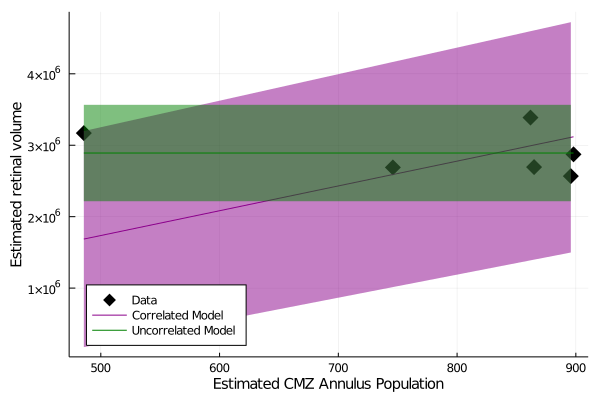
\includegraphics[width=.75\textwidth]{cmz/3dcorr.png}}    
    \caption{{\bf CMZ population and retinal volume estimates are uncorrelated at 3dpf}}
    Individual CMZ population estimate vs retinal volume estimate for 3dpf animals. Uncorrelated and correlated linear models of these variables are plotted as the mean$\pm$95\% CI of the predictive distribution of the fitted model. 
    Methods in \autoref{ssec:CMZpopvolest}, \autoref{ssec:CMZEmpBayes}.
    Code in \autoref{ssec:a10correlation}.
    \label{gausscorrelation}
\end{figure}


\subsection{Empirical Bayes linear regression}
\label{ssec:EmpiricalBayes}


\subsection{Galilean Monte Carlo}
\label{ssec:GMC}
Galilean Monte Carlo (GMC) is an algortihm for the \autoref[ssec:MonteCarlo]{sequential Monte Carlo} generation of new sample proposals within a parameter space. While GMC was introduced in 2012 \cite{Skilling2012}, the algorithm used in \ref{chap:GMC} is Skillings' 2019 revision \cite{Skilling2019}, which prevents model-particles from leaving the likelihood contour in order to find a reflection, and adds an additional reflection direction. 

GMC operates by assigning model-particles (ie. a particular parameterisation of that model at some point in parameter space) a velocity vector, chosen isotropically (ie. uniformly, without preference for any direction). New proposals are generated by moving the particle along the velocity vector. A proposed position's likelihood is calculated, and the proposal is accepted if this value is greater than or equal to the contour. $\geq$ is required to allow particles to search likelihood "plateaus", which are prominently seen in the models of \ref{chap:CNS}, due to the discretised (timepoint-bound) nature of the observations.

If a proposal is rejected, its current vector crosses the likelihood contour at a distance less than that of the proposal. If this occurs, the particle reflects off the boundary and carries on down the reflected vector with the same velocity. Nothing about the likelihood measure is used to propose positions, so it samples evenly from within the likelihood contour, fulfilling detailed balance \cite{Skilling2012}. This means that particles are equally likely to transition between positions in the forward process as the reverse process; in GMC the proposal process to move up-vector is identical to the one to move down vector, should the particle reflect normal to the boundary.

When a reflection is being proposed, samples are sequentially taken in three ``directions'', with the first of these to be accepted, used as the reflected model-particle. The three new vectors are produced by

\begin{enumerate}
    \item 
\end{enumerate}

\subsection{Nested sampling}
\label{ssec:nested}
Nested sampling is an algorithmic process for estimating the quality of a model, given observations. It arises from fundamental considerations of imposing a measure on statements about a model of a phenomenon \cite{Skilling2012}. The most basic such statement is an atomic true/false proposition. A measure is a function that assigns a value to a set. A measure of a model's evidence values a statement or a set of statements about the model, given some observations. A set of statements about the world can be represented as a boolean lattice of the statements and their OR combinations \cite{Knuth2012}. The sum and product rules arise in combining measures assigned to these statements into measures of their sets: ie. the probability of A OR B is $p(A) + p(B)$, while the probability of A AND B is $p(A) \times p(B)$. These operators are required in order to preserve consistent ordering between measures and their combinations. This lattice-oriented view thus gives rise to a unique calculus for measuring the divergence of model output from observations over sets of model-propositions\cite{Knuth2012}. The uniqueness, basic symmetry, and non-arbitrary nature of the axioms underlying nested sampling strongly suggest that this approach is fundamentally superior to other, more ad hoc methods of estimating model quality (eg. \hyperref[ssec:AIC]{AIC}).





\subsection{Expectation Maximization optimization of HMMs}
\label{ssec:EM}
In order to select appropriate background models for \textit{D. rerio} genomic noise in \autoref{chap:rys}, 
